\documentclass[chaptersright]{informeutn}
\usepackage[table]{xcolor}
\usepackage{listings}
\usepackage{pdfpages}
\usepackage{tikz/tikzit}
\usepackage{wrapfig}

\input{tikz/TikZiT_style.tikzstyles}

\lstdefinestyle{ltspice}{
  backgroundcolor=\color{gray!10},
  basicstyle=\ttfamily\small,
  keywordstyle=\color{blue},
  commentstyle=\color{green!50!black},
  stringstyle=\color{orange},
  frame=single,
  breaklines=true,
  postbreak=\mbox{\textcolor{red}{$\hookrightarrow$}\space},
  columns=flexible,
  captionpos=b
}
\renewcommand{\lstlistingname}{Listado}

% Datos del informe
\materia{Dispositivos Electronicos}
\titulo{Trabajo Práctico 5}
\comision{3R2}
\autores{
          Santino Noccetti, 405927 - Operario y Documentador\\
          Franco Palombo, 401910 - Coordinador}
\fecha{01/01/2001}

\begin{document}
  \maketitle

  \tableofcontents
  \setcounter{page}{1}
  \thispagestyle{plain}

  \chapter{Introducción}
En el presente trabajo práctico se estudian las características eléctricas del transistor de efecto de campo de juntura
(JFET), dispositivo ampliamente utilizado en aplicaciones analógicas por su alta impedancia de entrada y su capacidad de
control mediante voltaje. 

El objetivo principal es comprender el comportamiento del JFET en sus distintas regiones de operación (saturación y
corte) a partir de simulaciones realizadas en LTSpice y de experiencias de laboratorio con el transistor 2N5457. 

A lo largo del informe se analizan las curvas características de salida y de transferencia, así como los parámetros
fundamentales del dispositivo, tales como la corriente de saturación $I_{DSS}$ y la tensión de corte $V_{GS(off)}$.
Finalmente, se realiza una comparación entre los resultados experimentales, los obtenidos por simulación y los datos
proporcionados en la hoja de datos del fabricante, con el fin de evaluar la precisión de los modelos y afianzar los
conceptos teóricos desarrollados en clase.

  \chapter{Rectificador Controlado de Silicio}
  \begin{wrapfigure}{R}{0.3\textwidth}
  \vspace{-1cm}
    \centering
    \resizebox{!}{\linewidth}{
    \begin{tikzpicture}
	\begin{pgfonlayer}{nodelayer}
		\node [style=none] (0) at (-1, 2) {};
		\node [style=none] (1) at (1, 2) {};
		\node [style=none] (2) at (-1, 1) {};
		\node [style=none] (3) at (1, 1) {};
		\node [style=none] (4) at (-1, 0) {};
		\node [style=none] (5) at (1, 0) {};
		\node [style=none] (6) at (-1, -1) {};
		\node [style=none] (7) at (1, -1) {};
		\node [style=none] (8) at (-1, -2) {};
		\node [style=none] (9) at (1, -2) {};
		\node [style=none] (10) at (-0.5, -2) {};
		\node [style=none] (11) at (0.5, -2) {};
		\node [style=none] (12) at (-0.5, -2.25) {};
		\node [style=none] (13) at (0.5, -2.25) {};
		\node [style=none] (14) at (-0.5, 2.25) {};
		\node [style=none] (15) at (0.5, 2.25) {};
		\node [style=none] (16) at (-0.5, 2) {};
		\node [style=none] (17) at (0.5, 2) {};
		\node [style=none] (18) at (-1.25, -0.25) {};
		\node [style=none] (19) at (-1, -0.25) {};
		\node [style=none] (20) at (-1.25, -0.75) {};
		\node [style=none] (21) at (-1, -0.75) {};
		\node [style=none] (22) at (-1.25, -0.5) {};
		\node [style=none] (23) at (0, -2.25) {};
		\node [style=none] (24) at (0, 2.25) {};
		\node [style=none] (25) at (0, 3) {};
		\node [style=none] (26) at (-2, -0.5) {};
		\node [style=none] (27) at (0, -3) {};
		\node [style=none] (28) at (0, 1.5) {p};
		\node [style=none] (29) at (0, 0.5) {n};
		\node [style=none] (30) at (0, -0.5) {p};
		\node [style=none] (31) at (0, -1.5) {n};
		\node [style=none] (32) at (0, -3.25) {K};
		\node [style=none] (33) at (0, 3.25) {A};
		\node [style=none] (34) at (-2.25, -0.5) {G};
	\end{pgfonlayer}
	\begin{pgfonlayer}{edgelayer}
		\draw [style=fill2] (3.center)
			 to (2.center)
			 to (0.center)
			 to (1.center)
			 to cycle;
		\draw [style=fill2] (4.center)
			 to (6.center)
			 to (7.center)
			 to (5.center)
			 to cycle;
		\draw [style=fill3] (4.center)
			 to (5.center)
			 to (3.center)
			 to (2.center)
			 to cycle;
		\draw [style=fill3] (8.center)
			 to (9.center)
			 to (7.center)
			 to (6.center)
			 to cycle;
		\draw [style=fill4] (10.center)
			 to (12.center)
			 to (13.center)
			 to (11.center)
			 to cycle;
		\draw [style=fill4] (14.center)
			 to (16.center)
			 to (17.center)
			 to (15.center)
			 to cycle;
		\draw [style=fill4] (18.center)
			 to (20.center)
			 to (21.center)
			 to (19.center)
			 to cycle;
		\draw (22.center) to (26.center);
		\draw (24.center) to (25.center);
		\draw (23.center) to (27.center);
	\end{pgfonlayer}
\end{tikzpicture}

    }
    \caption{estructura interna del SCR.}
    \label{fig:scr_si}
  \end{wrapfigure}
  Un SCR (rectificador controlado de silicio, silicon-controlled rectifier) es un dispositivo pnpn de 4 capas similar al
  diodo de 4 capas pero con tres terminales: ánodo, cátodo y compuerta. En la figura \ref{fig:scr_si} puede ver la
  construcción básica del mismo, y su símbolo esquemático.

  \section{Activación del SCR}
    Cuando la corriente en la compuerta, $I_G$, es cero, por lo que el dispositivo actúa como un diodo de 4 capas en el
    estado de apagado. En este estado, la muy alta resistencia entre el ánodo y el cátodo pueden ser simulados de forma
    aproximada por un interruptor abierto. Cuando se aplica un pulso (disparo) positivo de corriente a la compuerta, el
    dispositivo se enciende, generando un camino de baja resistencia para permitir el flujo de corriente entre ánodo y
    cátodo. El SCR se puede activar también por voltaje entre ánodo y cátodo, ya que mientras que $I_G = 0$, el componente
    se comportara como un diodo de 4 capas.

    Se propuso analizar las regiones de acrivacion y corrientes de codo del SCR seleccionado y compararlas con las
    provistas por el fabricante en el datasheet. Para nuestra practica, seleccionamos el TYN612M. Para analizar las
    diferentes regiones, se realizaran 3 pruebas:
    \begin{itemize}
      \item Curva de $I_G = f_{(V_G)}$ para $V_{AK} = 0V$,
      \item Curva de $I_A = f_{(V_{AK})}$ para $V_G = 0V$,
      \item Curva de $I_A = f_{(V_G)}$ para $V_{AK} = 100V$.
    \end{itemize}

    Por cuestiones de seguridad, la curva de $I_A = f_{(V_{AK})}$ para $V_G = 0V$ solo se realizara en simulación.

    \subsection{Curva $I_G = f_{(V_G)}$}
      Para lograr esta curva, la única condición que se debe aplicar es mantener $V_{AK} = 0V$ en todo momento,
      mientras se varia el $V_G$.

      \subsubsection{Actividad de simulación}
        Se propuso realizar un barrido lineal de la tensión $V_G$ mientras que $V_{AK} = 0V$. El barrido es de $0V$ a
        $20V$ en pasos de $100mV$. Para trazar esta curva, el circuito utilizado es el de la figura \ref{crkt:scr_vak0}
        y los parámetros de simulación se pueden ver en \ref{list:scr_vak0}.
        \begin{figure}[!ht]
          \centering
          \begin{minipage}{0.45\textwidth}
            \centering
            \begin{tikzpicture}
	% Paths, nodes and wires:
	\draw (0, 2.3) to[american voltage source, l={$V_1$}] (0, -0);
	\draw (6.77, 4.5) to[american voltage source, l={$V_2$}] (6.77, 2.5);
	\draw (0, 2.3) to[american resistor, l={$4K7$}] (3, 2.3);
	\draw (3.77, 4) to[american resistor, l={$4K7$}] (3.77, 7);
	\draw (3.77, 4) to[empty thyristor, mirror] (3.77, 2);
	\draw (6.77, 4.5) -- (6.77, 7) -- (3.77, 7);
	\draw (3.77, 2) -| (3.77, -0) -- (6.77, -0) -| (6.77, 2.5);
	\draw (0, -0) -- (0.02, -0) -- (3.77, -0);
	\draw (3, 2.3) to[qvprobe, l_={$V_G$}] (3, -0);
\end{tikzpicture}
            \caption{circuito del SCR a simular}
            \label{crkt:scr_vak0}
          \end{minipage}
          \hfill
          \begin{minipage}{0.45\textwidth}
            \centering
          \begin{lstlisting}[style=ltspice, caption={Parámetros de simulación LTspice}, label=list:scr_vak0]
.dc V1 0 20 100m
          \end{lstlisting}
          \end{minipage}
        \end{figure}

      Revise la sección \ref{annex:scr_model} para ver el modelo SPICE utilizado para las simulaciones.
      \begin{figure}[!ht]
        \begin{tikzpicture}
          \begin{axis}[
            width=14cm,
            height=5.5cm,
            xlabel={$V_G$ [mV]},
            ylabel={$I_G$ [mA]},
            grid=both,
            minor tick num=1,
            scale only axis,
            enlargelimits=false,
              title={$I_G = f_{(V_G)}$},
            extra x ticks={550},
            extra x tick style={
              grid style={red, thick, dashed},
              tick style={red},
              tick label style={red}
             },
            scaled ticks=false,
            restrict x to domain=0:800,
            xmin=0, xmax=800
          ]
          \addplot[
            color=blue,
            mark=none,
            thick,
          ] table[
            col sep=tab,
            header=true,
            x expr=\thisrow{V(vg)}*1000,
            y expr=\thisrow{Ix(U1:G)}*1000
          ] {simulations/ig_vg_vak0.txt};
          \end{axis}
        \end{tikzpicture}
          \caption{gráfica de la corriente de gate en función de la tensión de gate.}
          \label{graph:scr_ig_vg_vak0}
      \end{figure}

      La curva relevada se puede ver en la figura \ref{graph:scr_ig_vg_vak0}, y esta es bastante similar a la curva de
      un diodo, con el cambio de que el potencial en el que empieza a conducir es menor. Esto se debe a que la unión
      presente entre gate y cátodo es, a los ojos del circuito de gate, un simple diodo.

      \subsubsection{Actividad de Laboratorio}
        Para esta actividad, en vez de variar la fuente, esta se mantuvo fija, y usando un potenciómetro fuimos variando
        su resistencia, provocando un cambio en la $V_G$ y la $I_G$. El circuito utilizado se puede ver en la figura
        \ref{crkt:scr_vak0_lab}.

        \begin{figure}[!ht]
          \centering
          \begin{minipage}{0.7\textwidth}
            \centering
            \resizebox{1\textwidth}{!}{
            \begin{tikzpicture}
	% Paths, nodes and wires:
	\draw (0.56, 2.3) to[american resistor, l={$4K7$}] (3.56, 2.3);
	\draw (7.83, 4) to[american resistor, l={$4K7$}] (7.83, 7);
	\draw (7.83, 4) to[empty thyristor, mirror] (7.83, 2);
	\draw (3.56, 2.3) to[qiprobe, l={$I_G$}] (5.56, 2.3);
	\draw (3.56, 2.3) to[qvprobe, l={$V_G$}] (3.56, -0);
	\draw (7.83, 2) to[qiprobe, l={$I_A$}] (7.83, -0);
	\draw (5.56, 2.3) to[normal open switch, l={$SW_1$}] (7.06, 2.3);
	\draw (10.06, 4) to[qvprobe, l_={$V_{AK}$}] (10.06, -0);
	\draw (11.06, 7) to[qvprobe, l={$V_i$}] (11.06, -0);
	\draw (0, 3.925) to[american potentiometer, l_={$5K$}] (0, 0.675);
	\draw (0, 0.675) |- (3.56, -0);
	\draw (3.56, -0) -- (7.83, -0) -- (10.06, -0) -- (11.06, -0);
	\node[vcc](N1) at (0, 7){} node[anchor=south] at (N1.text){$+20V$};
	\node[vcc](N2) at (7.83, 7){} node[anchor=south] at (N2.text){$V_i$};
	\draw (11.06, 7) |- (7.83, 7);
	\draw (10.06, 4) |- (7.83, 4);
	\draw (0, 7) -- (0, 3.925);
	\node[ground] at (7.83, -0){};
\end{tikzpicture}
            }
            \caption{circuito a implementar en el laboratorio.}
            \label{crkt:scr_vak0_lab}
          \end{minipage}
          \hfill
          \begin{minipage}{0.25\textwidth}
            \centering
            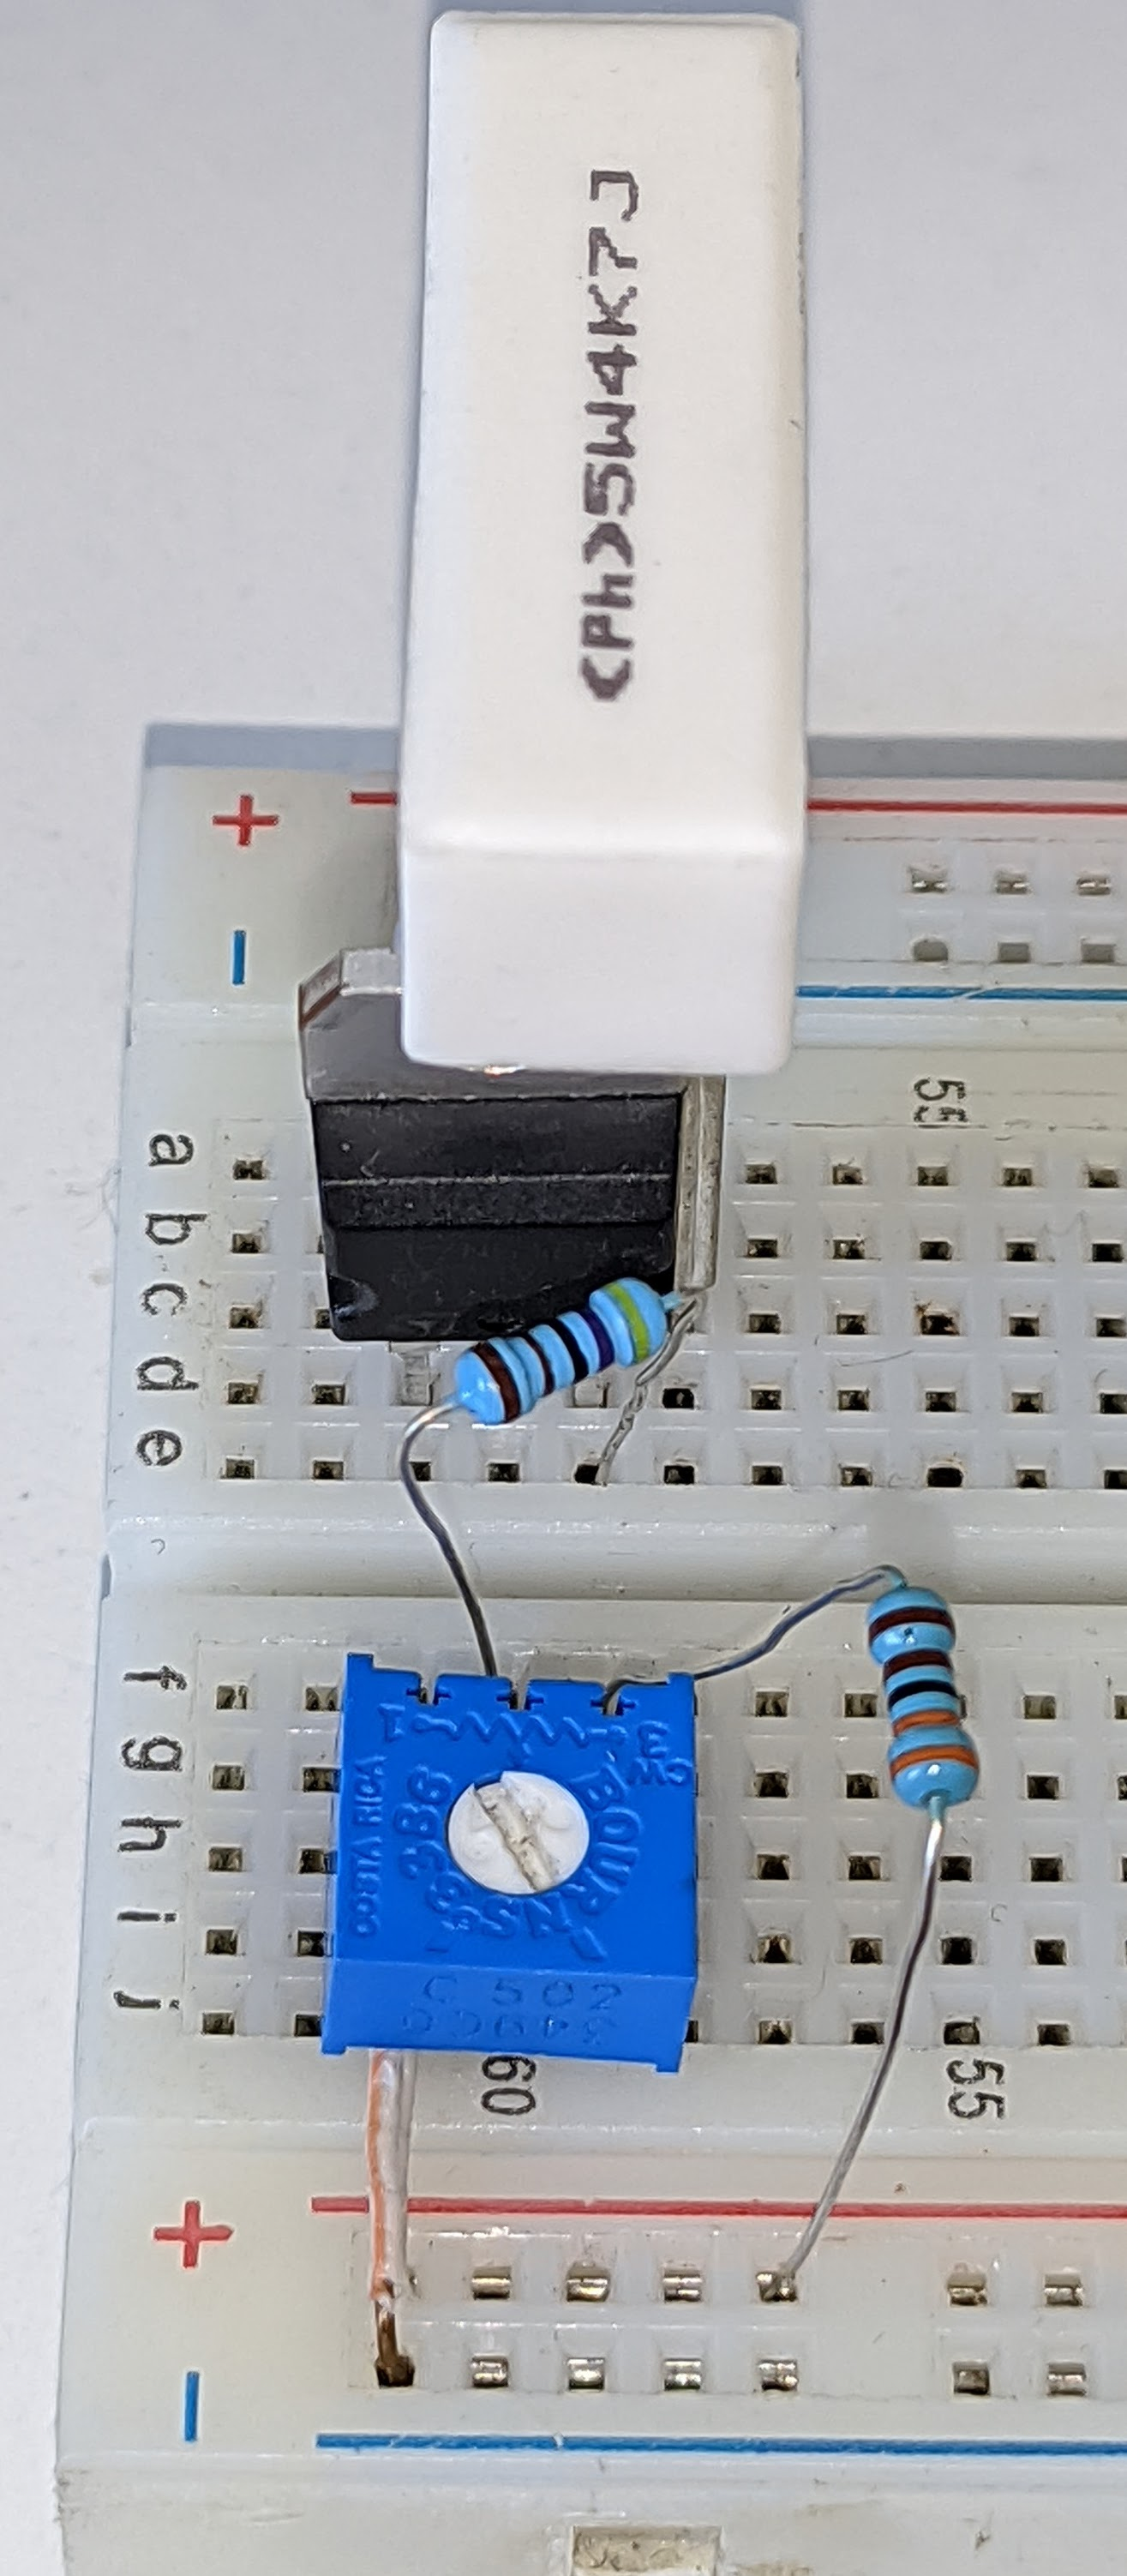
\includegraphics[width=0.8\textwidth]{pictures/prot_scr.jpg}
            \caption{circuito implementado en el laboratorio.}
          \end{minipage}
        \end{figure}

        Los datos relevados en el laboratorio se pueden ver en la tabla \ref{tab:scr_vak0_lab} y en la figura
        \ref{graph:scr_ig_vg_vak0_lab}. La curva es muy similar a la del diodo, solo que con un potencial de
        conducción mas bajo que el diodo común de silicio.

        \begin{figure}[!ht]
          \centering
          \begin{minipage}{0.3\textwidth}
            \centering
            \begin{tabular}{c|c}
              $V_G$ & $I_G$ \\ \hline
              0     & 0     \\
            \end{tabular}
            \caption{datos relevados en el laboratorio}
            \label{tab:scr_vak0_lab}
          \end{minipage}
          \hfill
          \begin{minipage}{0.6\textwidth}
            \begin{tikzpicture}
              \begin{axis}[
                width=8cm,
                height=5.5cm,
                xlabel={$V_G$ [mV]},
                ylabel={$I_G$ [mA]},
                grid=both,
                minor tick num=1,
                scale only axis,
                enlargelimits=false,
                  title={$I_G = f_{(V_G)}$},
                extra x ticks={550},
                extra x tick style={
                  grid style={red, thick, dashed},
                  tick style={red},
                  tick label style={red}
                 },
                scaled ticks=false,
                restrict x to domain=0:800,
                xmin=0, xmax=800
              ]
              \addplot[
                color=blue,
                mark=none,
                thick,
              ] table[
                col sep=tab,
                header=true,
                x expr=\thisrow{V(vg)}*1000,
                y expr=\thisrow{Ix(U1:G)}*1000
              ] {simulations/ig_vg_vak0.txt};
              \end{axis}
            \end{tikzpicture}
            \caption{gráfica $I_G = f_{(V_G)}$ relevada en el laboratorio.}
            \label{graph:scr_ig_vg_vak0_lab}
          \end{minipage}
        \end{figure}

      \subsection{Curva $I_A = f_{(V_{AK})}$}
        Para lograr esta curva, la única condición que se debe aplicar es mantener $V_G = 0V$ en todo momento,
        mientras se varia el $V_{AK}$.
          Se propuso realizar un barrido lineal de la tensión $V_{AK}$ mientras que $V_G = 0V$. El barrido es de $0V$ a
          $800V$ en pasos de $10V$. Para trazar esta curva, el circuito utilizado es el de la figura \ref{crkt:scr_vg0}
          y los parámetros de simulación se pueden ver en \ref{list:scr_vg0}.
          \begin{figure}[!ht]
            \centering
            \begin{minipage}{0.45\textwidth}
              \centering
              \begin{tikzpicture}
	% Paths, nodes and wires:
	\draw (0, 2.3) to[american voltage source, l={$V_1$}] (0, -0);
	\draw (6.77, 4.5) to[american voltage source, l={$V_2$}] (6.77, 2.5);
	\draw (0, 2.3) to[american resistor, l={$4K7$}] (3, 2.3);
	\draw (3.77, 4) to[american resistor, l={$4K7$}] (3.77, 7);
	\draw (3.77, 4) to[empty thyristor, mirror] (3.77, 2);
	\draw (6.77, 4.5) -- (6.77, 7) -- (3.77, 7);
	\draw (3.77, 2) -| (3.77, -0) -- (6.77, -0) -| (6.77, 2.5);
	\draw (0, -0) -- (0.02, -0) -- (3.77, -0);
	\draw (5.25, 4) to[qvprobe, l={$V_{AK}$}] (5.25, -0);
	\draw (5.25, 4) |- (3.77, 4);
\end{tikzpicture}
              \caption{circuito del SCR a simular}
              \label{crkt:scr_vg0}
            \end{minipage}
            \hfill
            \begin{minipage}{0.45\textwidth}
              \centering
            \begin{lstlisting}[style=ltspice, caption={Parámetros de simulación LTspice}, label=list:scr_vg0]
.dc V2 0 800 10
            \end{lstlisting}
            \end{minipage}
          \end{figure}

          \begin{figure}[!ht]
            \begin{tikzpicture}
              \begin{axis}[
                width=14cm,
                height=5.5cm,
                xlabel={$V_{AK}$ [V]},
                ylabel={$I_{AK}$ [mA]},
                grid=both,
                minor tick num=1,
                scale only axis,
                enlargelimits=false,
                  title={$I_{AK} = f_{(V_{AK})}$},
                extra x ticks={615},
                extra x tick style={
                  grid style={red, thick, dashed},
                  tick style={red},
                  tick label style={red}
                 },
                extra y ticks={140},
                extra y tick style={
                  grid style={red, thick, dashed},
                  tick style={red},
                  tick label style={red}
                 },
                scaled ticks=false,
                restrict x to domain=0:700,
                xmin=0, xmax=700
              ]
              \addplot[
                color=blue,
                mark=none,
                thick,
              ] table[
                col sep=tab,
                header=true,
                x expr=\thisrow{V(va)},
                y expr=\thisrow{Ix(U1:A)}*1000
              ] {simulations/iak_vak_vg0.txt};
              \end{axis}
            \end{tikzpicture}
              \caption{gráfica de la corriente de ánodo en función de la tensión ánodo-cátodo.}
              \label{graph:scr_iak_vak_vg0}
          \end{figure}

          Como se puede ver en la figura \ref{graph:scr_iak_vak_vg0}, la curva obtenida tiene cierta similitud a la
          curva teórica del SCR y del diodo de 4 capas. Lo que es un poco extraño es la $I_H$, que parece estar
          bastante mas alta que la especificada por la hoja de datos ($20mA$).
          %hay que ver de corregir el modelo. La IH es altisima comparada con la de la hoja de datos (approx 20mA)

    \subsection{Curva $I_A = f_{(V_G)}$}
      Para esta curva, se fijara $V_{AK} = 100V$ y haciendo un barrido lineal de $V_G$ trazaremos la curva y
      encontraremos el punto donde el SCR se dispara por corriente de gate.

      \subsubsection{Actividad de Simulación}
        Se propuso realizar un barrido lineal de la tensión $V_g$ mientras que $V_{AK} = 100V$. El barrido es de $0V$ a
        $20V$ en pasos de $100mV$. Para trazar esta curva, el circuito utilizado es el de la figura \ref{crkt:scr_vak100}
        y los parámetros de simulación se pueden ver en \ref{list:scr_vak100}.
        \begin{figure}[!ht]
          \centering
          \begin{minipage}{0.45\textwidth}
            \centering
            \begin{tikzpicture}
	% Paths, nodes and wires:
	\draw (0, 2.3) to[american voltage source, l={$V_1$}] (0, -0);
	\draw (6.77, 4.5) to[american voltage source, l={$V_2$}] (6.77, 2.5);
	\draw (0, 2.3) to[american resistor, l={$4K7$}] (3, 2.3);
	\draw (3.77, 4) to[american resistor, l={$4K7$}] (3.77, 7);
	\draw (3.77, 4) to[empty thyristor, mirror] (3.77, 2);
	\draw (6.77, 4.5) -- (6.77, 7) -- (3.77, 7);
	\draw (3.77, 2) -| (3.77, -0) -- (6.77, -0) -| (6.77, 2.5);
	\draw (0, -0) -- (0.02, -0) -- (3.77, -0);
	\draw (3, 2.3) to[qvprobe, l_={$V_G$}] (3, -0);
	\draw (5.25, 4) to[qvprobe, l={$V_{AK}$}] (5.25, 0);
	\draw (5.25, 4) |- (3.77, 4);
\end{tikzpicture}
            \caption{circuito del SCR a simular}
            \label{crkt:scr_vak100}
          \end{minipage}
          \hfill
          \begin{minipage}{0.45\textwidth}
            \centering
          \begin{lstlisting}[style=ltspice, caption={Parámetros de simulación LTspice}, label=list:scr_vak100]
.dc V1 0 20 100m
          \end{lstlisting}
          \end{minipage}
        \end{figure}

        \begin{figure}[!ht]
          \begin{tikzpicture}
            \begin{axis}[
              width=14cm,
              height=5.5cm,
              xlabel={$V_G$ [mV]},
              ylabel={$I_{AK}$ [mA]},
              grid=both,
              minor tick num=1,
              scale only axis,
              enlargelimits=false,
                title={$I_{AK} = f_{(V_G)}$},
              scaled ticks=false,
              restrict x to domain=0:700,
              xmin=0, xmax=700
            ]
            \addplot[
              color=blue,
              mark=none,
              thick,
            ] table[
              col sep=tab,
              header=true,
              x expr=\thisrow{V(vg)}*1000,
              y expr=\thisrow{Ix(U1:A)}*1000
            ] {simulations/iak_vg_vak100.txt};
            \end{axis}
          \end{tikzpicture}
            \caption{gráfica de la corriente de ánodo en función de la tensión de gate.}
            \label{graph:scr_iak_vg_vak100}
        \end{figure}

        %hay que concluir algo pero el modelo todavia no esta lo suficientemente pulido para generar esta curva de
        %manera adecuada

      \subsubsection{Actividad de Laboratorio}
        Nuevamente, para realizar la variación de la tensión de gate, se hizo lo mismo que para la actividad anterior,
        esto es, dejar fijo el voltaje de gate, y con un potenciómetro ir variando su resistencia y con el su voltaje.
        El circuito empleado es el mismo de la figura \ref{crkt:scr_vak0_lab}.

        Como primer apartado, fijando la $V_{AK} = 100V$ fuimos variando el potenciómetro hasta que notamos que el
        dispositivo se activo por corriente de gate. Los valores relevados son:
        \begin{equation*}
          V_G = \quad I_G =
        \end{equation*}

        Posterior a eso, desconectamos el circuito de disparo y notamos que el dispositivo permaneció en la región de
        conducción. Esto es porque la corriente $I_{AK} > I_H$. Posterior a esa prueba, fuimos bajando $V_{AK}$ para
        encontrar cual era la $I_H$ para un $V_G = 0V$. Los datos relevados en el laboratorio se pueden ver en la tabla
        \ref{tab:scr_vak100_lab} y en la figura \ref{graph:scr_ig_vg_vak100_lab}. 

        \begin{figure}[!ht]
          \centering
          \begin{minipage}{0.3\textwidth}
            \centering
            \begin{tabular}{c|c}
              $V_{AK}$ & $I_{AK}$ \\ \hline
              0     & 0     \\
            \end{tabular}
            \caption{datos relevados en el laboratorio}
            \label{tab:scr_vak100_lab}
          \end{minipage}
          \hfill
          \begin{minipage}{0.6\textwidth}
            \begin{tikzpicture}
              \begin{axis}[
                width=8cm,
                height=5.5cm,
                xlabel={$V_{AK}$ [mV]},
                ylabel={$I_{AK}$ [mA]},
                grid=both,
                minor tick num=1,
                scale only axis,
                enlargelimits=false,
                  title={$I_{AK} = f_{(V_G)}$},
                extra x ticks={550},
                extra x tick style={
                  grid style={red, thick, dashed},
                  tick style={red},
                  tick label style={red}
                 },
                scaled ticks=false,
                restrict x to domain=0:800,
                xmin=0, xmax=800
              ]
              \addplot[
                color=blue,
                mark=none,
                thick,
              ] table[
                col sep=tab,
                header=true,
                x expr=\thisrow{V(vg)}*1000,
                y expr=\thisrow{Ix(U1:A)}*1000
              ] {simulations/iak_vg_vak100.txt};
              \end{axis}
            \end{tikzpicture}
            \caption{gráfica $I_{AK} = f_{(V_{AK})}$ relevada en el laboratorio.}
            \label{graph:scr_ig_vg_vak100_lab}
          \end{minipage}
        \end{figure}

        Después de haber logrado apagar el dispositivo haciendo que $I_{AK} < I_H$, procedimos a poner $V_{AK} = 100V$.
        El dispositivo permaneció sin polarización hasta que el circuito de disparo, que quedo con la tensión y
        corriente de disparo, fue conectado, lo que genero que el dispositivo se polarice y comience a circular
        corriente. El comportamiento es idéntico al previamente mencionado.

        Por ultimo, se realizo la prueba de que el SCR quede colocado en inversa, y generar la misma corriente de
        disparo al mismo voltaje. En este caso, no hubo circulación de corriente apreciable, incluso después de subir la
        corriente de gate, por lo que en inversa, el SCR se sigue comportando como un diodo de 4 capas,
        independientemente de la corriente presente en gate.

  \section{Curva característica del SCR}
    Con la información relevada anteriormente respecto a la activación del SCR, podemos ahora pasar a recrear las curvas
    características del SCR. Para ello, la idea es fijar una corriente de gate, e ir haciendo un barrido de la $V_{AK}$
    hasta encontrar el $V_{BR(Fn)}$, voltaje en el cual el dispositivo se polariza y comienza a conducir. El circuito
    implementado en el laboratorio, es el mismo que se utilizo anteriormente. Puede verlo en la figura
    \ref{crkt:scr_curvcar_lab}.

    \begin{figure}[!ht]
      \centering
      \begin{tikzpicture}
	% Paths, nodes and wires:
	\draw (0.56, 2.3) to[american resistor, l={$4K7$}] (3.56, 2.3);
	\draw (7.83, 4) to[american resistor, l={$4K7$}] (7.83, 7);
	\draw (7.83, 4) to[empty thyristor, mirror] (7.83, 2);
	\draw (3.56, 2.3) to[qiprobe, l={$I_G$}] (5.56, 2.3);
	\draw (3.56, 2.3) to[qvprobe, l={$V_G$}] (3.56, -0);
	\draw (7.83, 2) to[qiprobe, l={$I_A$}] (7.83, -0);
	\draw (5.56, 2.3) to[normal open switch, l={$SW_1$}] (7.06, 2.3);
	\draw (10.06, 4) to[qvprobe, l_={$V_{AK}$}] (10.06, -0);
	\draw (11.06, 7) to[qvprobe, l={$V_i$}] (11.06, -0);
	\draw (0, 3.925) to[american potentiometer, l_={$5K$}] (0, 0.675);
	\draw (0, 0.675) |- (3.56, -0);
	\draw (3.56, -0) -- (7.83, -0) -- (10.06, -0) -- (11.06, -0);
	\node[vcc](N1) at (0, 7){} node[anchor=south] at (N1.text){$+20V$};
	\node[vcc](N2) at (7.83, 7){} node[anchor=south] at (N2.text){$V_i$};
	\draw (11.06, 7) |- (7.83, 7);
	\draw (10.06, 4) |- (7.83, 4);
	\draw (0, 7) -- (0, 3.925);
	\node[ground] at (7.83, -0){};
\end{tikzpicture}
      \caption{circuito a implementar en el laboratorio.}
      \label{crkt:scr_curvcar_lab}
    \end{figure}

    \begin{table}[!ht]
      \centering
      \begin{tabular}{c|c|c|c|c|c|c|c|c|c}
        \multicolumn{2}{c|}{$I_G = mA$} & \multicolumn{2}{c|}{$I_G = mA$} & \multicolumn{2}{c|}{$I_G = mA$} & \multicolumn{2}{c|}{$I_G = mA$} & \multicolumn{2}{c}{$I_G = mA$} \\
        $V_{AK}$ & $I_{AK}$ & $V_{AK}$ & $I_{AK}$ & $V_{AK}$ & $I_{AK}$ & $V_{AK}$ & $I_{AK}$ & $V_{AK}$ & $I_{AK}$ \\ \hline
        
      \end{tabular}
      \caption{valores relevados en el laboratorio.}
      \label{tab:scr_curvcar_lab}
    \end{table}

    \begin{figure}[!ht]
      \begin{tikzpicture}
        \begin{axis}[
          width=14cm,
          height=5.5cm,
          xlabel={$V_G$ [mV]},
          ylabel={$I_{AK}$ [mA]},
          grid=both,
          minor tick num=1,
          scale only axis,
          enlargelimits=false,
            title={$I_{AK} = f_{(V_G)}$},
          scaled ticks=false,
          restrict x to domain=0:700,
          xmin=0, xmax=700
        ]
        \addplot[
          color=blue,
          mark=none,
          thick,
        ] table[
          col sep=tab,
          header=true,
          x expr=\thisrow{V(vg)}*1000,
          y expr=\thisrow{Ix(U1:A)}*1000
        ] {simulations/iak_vg_vak100.txt};
        \end{axis}
      \end{tikzpicture}
      \caption{familia de curvas de $I_{AK} = f_{V_{AK}, I_G}$}
      \label{graph:scr_curvcar_lab}
    \end{figure}

    Puede revisar los valores relevados en el laboratorio en la tabla \ref{tab:scr_curvcar_lab} y la familia de curvas
    en la figura \ref{graph:scr_curvcar_lab}. Las tablas terminan cuando en el recorrido de tensión a la próxima
    medición generaba el disparo.

  \section{SCR en Corriente Alterna}


  \chapter{DIAC}

  \section{Reversibilidad del DIAC}

  \chapter{TRIAC}

  \section{Curva característica del TRIAC}

  \section{Recortador de onda con TRIAC}

  \chapter{Interpretación de hojas de datos}

  \chapter{Conclusiones}
Este trabajo práctico se centró en el análisis del transistor de efecto de campo de juntura (JFET), un
componente fundamental dentro de la electrónica analógica y de potencia. El JFET, por su estructura y
principio de funcionamiento, permite comprender cómo el control de una unión polarizada en inversa
afecta directamente la conducción de corriente a través de un canal semiconductor, lo que lo convierte
en un dispositivo idóneo para aplicaciones de conmutación y amplificación.  

El objetivo principal del trabajo fue caracterizar experimental y teóricamente las distintas regiones 
de operación del JFET, abarcando desde el corte hasta la saturación, así como la zona óhmica 
intermedia. Para ello, se diseñaron e implementaron circuitos en un entorno de simulación (LTSpice) 
y posteriormente se replicaron en el laboratorio utilizando instrumental básico como fuentes de 
alimentación, multímetros y protoboard.  

Durante la práctica se obtuvieron curvas características $I_{DS} = f(V_{DS})$ para diferentes valores 
de $V_{GS}$, lo que permitió observar el efecto del voltaje de compuerta sobre la corriente de drenaje. 
Asimismo, se determinó la corriente de saturación $I_{DSS}$, el voltaje de estrangulamiento 
$V_{GS(off)}$ y la característica de transferencia universal, parámetros esenciales para describir 
matemáticamente el comportamiento del dispositivo.  

La comparación entre los datos experimentales, los resultados de simulación y los valores provistos 
por el fabricante en la hoja de datos permitió no solo validar los modelos teóricos, sino también 
identificar discrepancias atribuibles a tolerancias de fabricación, condiciones de medición y 
limitaciones propias de los modelos idealizados. Esta integración entre teoría, simulación y práctica 
resulta esencial para consolidar un aprendizaje completo sobre el funcionamiento real de los 
semiconductores.   

  \chapter{Anexos}
  \section{Rubrica}
\begin{figure}[!h]
  \centering
  \begin{tabular}[c]{|c|c|c|}
    \rowcolor{gray!30}
    \hline
    \textbf{Tarea}                      & \textbf{Puntuación} & \textbf{Máximo}\\
    \hline
    Presentación del informe            &                     & 30\%\\
    \hline
    Explicación del proceso de medición &                     & 40\%\\
    \hline
    Defensa de las conclusiones         &                     & 30\%\\
    \hline
    \textbf{Total}                      &                     & \textbf{100\%}\\
    \hline
  \end{tabular}
\end{figure}

\section{Planilla de Seguimiento}
\begin{figure}[!h]
  \begin{footnotesize}
    \begin{tabular}{|m{1cm}|m{1cm}|m{1.3cm}|m{2cm}|m{1.7cm}|m{1.7cm}|m{1.7cm}|m{1.7cm}|m{1.7cm}|}
      \hline
      Versión del TP & Fecha de Inicio & Revisado Por & Resumen Observaciones Correcciones &
      Fecha de retroalimentación enviada & Cambios realizados por JTP? & Nueva fecha de entrega &
      Aprobado por jefe de cátedra?\\
      \hline
      1.0 (2025) & & & & & & &\\
      \hline
    \end{tabular}
  \end{footnotesize}
\end{figure}
 

  \section{Modelos SPICE}
    \lstinputlisting[style=ltspice, caption={Modelo SPICE del TYN612M},
    label=annex:scr_model]{simulations/models/tny612m.lib}
 
  \section{Hojas de Datos}
    \includepdf[pages=1]{annex/bt137x.pdf}
    \includepdf[pages=1]{annex/db3.pdf}
    \includepdf[pages=1]{annex/tyn612m.pdf}


\end{document}
